\documentclass[
  manuscript=article,  
  layout=preprint,  
  year=2023,
  volume=0,
]{format}

\usepackage{soul}
\usepackage{gensymb}

% --- blew is the area for authors ---

\usepackage[english]{babel}
\usepackage{comment}

% specify the .bib file for references
\addbibresource{reference.bib} 

% Make sure your article tile is within 12 words
\title{Dependencia espacial en la evaluación de la susceptibilidad por movimientos en masa}

\author{Edier Aristizábal}
\affiliation{Departamento de Geociencias y Medio Ambiente, Universidad Nacional de Colombia, Medellín, Colombia}

% maximum five keywords
\keywords{landslide; susceptibility; spatial dependence} 

\begin{document}

\begin{abstract}
Landslides are critical geomorphological processes that substantially reshape the landscape through the downslope movement of soil and rock, often triggered by factors such as rainfall, earthquake, or anthropogenic interventions. These processes pose significant hazards to infrastructure, human safety, and socioeconomic stability. Conventional statistical models frequently fail to adequately capture the spatial nature of landslide susceptibility assessment, often leading to biased or misleading outcomes due to the assumption of independence among observations, which ignores inherent spatial heterogeneity and spatial dependence. This study addresses these limitations by employing Spatial Autoregressive Models (SAR), which explicitly account for spatial dependence through the integration of neighborhood matrices. The dataset comprises catchments from the Colombian Andes, incorporating morphometric predictors at both local and regional scales, including slope, hypsometry, basin area, and annual precipitation. We built a neighborhood matrix based on distance criteria, recognizing that geoenvironmental factors influencing landslides often extend beyond direct boundaries, requiring a broader understanding of spatial interactions. Our findings demonstrate that incorporating spatial dependence significantly enhances both the predictive accuracy and interpretative power of the models when compared to conventional approaches. Analysis using Moran's Index revealed that basin slope and precipitation exhibit strong spatial dependence, forming clusters of similar values, which underscores the necessity of accounting for spatial effects. The Spatial Durbin Error Model (SDEM) outperformed alternative models by providing higher adjusted $R^2$ values and optimizing the balance between model complexity and fit, as measured by the Akaike Information Criterion (AIC). By explicitly integrating spatial structure, this study provides a more robust and realistic assessment of landslide susceptibility, which is crucial for understanding and managing these hazards in regions like the Colombian Andes.

\end{abstract}

\section{Introducción}

Los movimientos en masa son procesos geomorfológicos transformadores del paisaje que corresponden al desprendimiento y desplazamiento de materiales, como suelo y roca, ladera abajo por efecto de la gravedad (\cite{soeters1996slope, brabb1984innovative}). Estos eventos pueden ser desencadenados por factores como precipitación, sismos o intervención antrópica (\cite{corominas2014recommendations, fell2008guidelines}). Dado lo anterior, la susceptibilidad por movimientos en masa se define como la probabilidad de ocurrencia de estos procesos en un área específica, lo cual es fundamental para identificar zonas potencialmente críticas y para tomar decisiones informadas en la gestión del territorio, la planificación urbana y la mitigación de desastres (\cite{brabb1984innovative, corominas2014recommendations}).

La evaluación de la susceptibilidad por movimientos en masa es, en esencia, un problema espacial que involucra un amplio número de variables geoambientales (\cite{reichenbach2018review}). Los movimientos en masa están directamente influenciados por el entorno donde ocurren, lo cual implica una estrecha relación con las características del terreno, así como con las áreas circundantes (\cite{soeters1996}). Es por esta razón, que los inventarios de movimientos en masa, así como de variables morfométricas del terreno, condiciones geológicas y ambientales, permiten inferir las condiciones bajo las cuales se desencadenaron los eventos en el pasado, para predecir la ocurrencia de futuros movimientos en masa, bajo el supuesto que procesos similares podrían ocurrir en el futuro bajo condiciones semejantes (\cite{dai2001assessment, soeters1996slope}).

La identificación, caracterización y mapeo de estas variables geoambientales, que condicionan la ocurrencia de movimientos en masa, permiten incorporar en los modelos de susceptibilidad los patrones espaciales en la distribución de la ocurrencia de movimientos en masa (\cite{reichenbach2018review}); lo que corresponde a un mapa de susceptibilidad. Una de las técnicas para establecer dichos patrones espaciales es a través de los métodos estadísticos, también denominados métodos basados en datos o recientemente aprendizaje de máquinas (\textit{machine learning}) (\cite{korup2014landslide}). Estos métodos se caracterizan por su capacidad de procesar grandes cantidades de datos y encontrar, mediante técnicas estadísticas, patrones que relacionan la variable respuesta (la ocurrencia o no de movimientos en masa) y las variables geoambientales incorporadas en el análisis como predictores.

Sin embargo, además de las variables geoambientales observables e incorporadas en los modelos de susceptibilidad, existen una serie de variables latentes, es decir que no pueden ser observadas o medidas directamente, pero que influye en el comportamiento de otras variables del modelo (\cite{lombardo2019geostatistical}). Algunas de ellas asociadas a las características espaciales de las variables. Este componente latente en algunas ocasiones está incorporado dentro de las variables predictoras, pero no es considerado o permitido en los modelos estadísticos clásicos (\cite{anselin1988spatial, cressie1988spatial, lesage2011pitfalls}). En otros casos, estos factores simplemente se omiten.

Para atender esta problemática es necesario inicialmente comprender la estructura espacial de los datos. La estructura espacial se puede descomponer en dos componentes principales: la heterogeneidad espacial y la dependencia espacial (\cite{anselin1996simple, rey2023geographic}). La heterogeneidad espacial se refiere a la variación en las propiedades de los datos en diferentes áreas del espacio, lo que implica que las relaciones entre las variables no necesariamente sean homogéneas en toda la región de estudio (\cite{rey2023geographic}). Por ejemplo, en una región montañosa como los Andes, las características geológicas y climáticas pueden variar significativamente de un lugar a otro, lo que puede generar que una variable tenga una influencia variable a lo largo de la zona de estudio en la ocurrencia de movimientos en masa. La dependencia espacial, por otro lado, se refiere a la tendencia de valores similares a agruparse espacialmente (\cite{anselin1988spatial}). Esto implica que el valor de una variable en un punto del espacio está correlacionado con los valores de la misma variable en puntos cercanos, un fenómeno también conocido como autocorrelación. Esta dependencia puede originarse debido a procesos naturales que presentan continuidad espacial, como la geología y la topografía, o debido a factores ambientales como la vegetación y el clima (\cite{samia2019dynamic, lombardo2020space}), que tienden a presentar patrones espaciales similares en áreas cercanas.

Cuando la heterogeneidad y la dependencia espacial no se incorporan adecuadamente en los modelos, la estructura espacial queda remanente en los residuales, lo cual se traduce en una falta de ajuste adecuada del modelo (\cite{anselin2022spatial, cressie2015statistics, }). Este remanente espacial en los residuos es una violación de las suposiciones de independencia que subyacen a los modelos clásicos, ya que los modelos clásicos suelen asumir que las observaciones son independientes entre sí (sin dependencia espacial) y que la relación entre las variables es constante en toda la región de estudio (sin heterogeneidad espacial) (\cite{lesage2011pitfalls, banerjee2008gaussian}). Esto afecta la validez de las inferencias estadísticas y resulta en modelos con predicciones sesgadas (\cite{cressie1988spatial}). 

Para incorporar la dependencia espacial en los modelos, se puede utilizar los llamados Modelos Autoregresivos Simultáneos (\cite{whittle1954stationary}), los cuales permiten modelar la dependencia espacial a través de la inclusión de una matriz de vecindad. Esta matriz define la estructura de los vecinos de cada unidad de mapeo, ya sea en función de la distancia entre unidades o a partir de relaciones de contigüidad (\cite{anselin1996simple, elhorst2014spatial}).

Los modelos SAR son ampliamente utilizados en econometría y geografía, así como en otros campos que requieren un análisis espacial riguroso, como la epidemiología y la planificación urbana (\cite{elhorst2022dynamic, rey2023geographic, jaya2021spatial, ver2018spatial}). Sin embargo, la aplicación de algunos de estos modelos requiere de técnicas especiales, ya que la estructura de dependencia espacial puede introducir complicaciones que no están presentes en los modelos estadísticos clásicos (\cite{anselin1990spatial}).

En este artículo presentamos el concepto de dependencia espacial, su influencia en la evaluación de la susceptibilidad por movimientos en masa y modelos estadísticos que nos permiten incorporar este componente espacial en la modelación. Para ello, se utiliza un conjunto de datos de movimientos en masa y cuencas ubicadas en los Andes colombianos. A través de este estudio, se evalúa la estructura espacial presente en los datos y se aplican modelos autoregresivos que permiten incorporar esta estructura de manera explícita. La incorporación de la dependencia espacial en los modelos de susceptibilidad no solo nos permite mejorar la capacidad predictiva de los modelos, sino que también ofrece una interpretación más realista de los factores que influyen en la ocurrencia de movimientos en masa.

\section{Modelos de Autoregresión Espacial}

Los modelos de autoregresión espacial son un tipo de modelo estadístico utilizado para capturar y modelar la dependencia espacial entre unidades de análisis geográficas (\cite{whittle1954stationary, getis2009spatial, stakhovych2009specification, ripley1988statistical}). En lugar de asumir que las observaciones son independientes entre sí, estos modelos reconocen que las unidades cercanas en el espacio tienden a presentar valores similares (\cite{anselin1988spatial}). 

La aplicabilidad de los modelos de autoregresión espacial en los estudios de susceptibilidad a movimientos en masa radica en la naturaleza inherentemente espacial de estos fenómenos. Los movimientos en masa tienden a estar influenciados por las condiciones de las áreas adyacentes, como el relieve del terreno, condiciones climáticas, la cobertura del suelo y las características geológicas (\cite{samia2019dynamic}). Estos modelos son ampliamente utilizados en análisis espaciales debido a su capacidad para incluir explícitamente la estructura de dependencia entre las unidades vecinas a través de matrices de vecindad (\cite{lesage2011pitfalls, kelejian2007relative}). Esta matriz introduce el componente espacial, permitiendo que el valor de la variable respuesta en cada unidad de análisis se vea influido por los valores de las unidades vecinas. Esto permite modelar explícitamente el efecto que tienen los vecinos en la variable de interés.

Sin embargo, los modelos de autoregresión espacial también presentan algunas limitaciones (\cite{lesage2011pitfalls, anselin2022spatial}). La estimación de los parámetros en los modelos de autoregresión espacial puede ser compleja, especialmente cuando se trabaja con grandes conjuntos de datos y matrices de vecindad densas. Adicionalmente, la definición de la matriz de vecindad es fundamental, y una elección incorrecta puede llevar a resultados sesgados o poco representativos.

Las matrices de vecindad son una pieza clave en los modelos de autoregresión espacial (\cite{earnest2007evaluating}). Una matriz de vecindad define qué unidades se consideran "vecinas" y cómo se relacionan entre sí. Cada elemento de la matriz representa la fuerza o presencia de una relación espacial entre dos unidades. Existen diferentes tipos de matrices de vecindad (\cite{earnest2007evaluating, getis2009spatial, stakhovych2009specification}):

1. \textbf{Matriz de Vecindad Basada en la Contigüidad}: Este tipo de matriz define como vecinos a aquellas unidades que comparten un límite común. Es ideal para el análisis en zonas divididas en celdas regulares o regiones administrativas.

2. \textbf{Matriz de Vecindad Basada en Distancia}: En este tipo de matriz, se consideran vecinos aquellas unidades que se encuentran dentro de un radio específico de distancia. La vecindad se define en términos de la cercanía física.

3. \textbf{Matriz de Vecindad K-Vecinos más Cercanos}: Esta matriz define como vecinos a un número fijo de las unidades más cercanas a cada unidad de análisis. Asegura que cada unidad tenga el mismo número de vecinos, lo cual puede ser útil para evitar problemas de unidades aisladas sin vecinos.

La ecuación básica de un modelo de autoregresión simultaneo se puede representar de la siguiente manera (\cite{cliff1981spatial, kelejian2007relative, lesage2009introduction}):

\begin{equation}
Y = \rho W Y + X \beta + \epsilon
\end{equation}

donde el término $\rho$ introduce el componente espacial, permitiendo que el valor de la variable respuesta \textbf{Y} en cada unidad de análisis esté influido por los valores de las unidades vecinas, ponderados por la matriz de vecindad (W). \textbf{$\beta$} es el vector de coeficientes de regresión asociados a las variables predictoras (X). Estos coeficientes reflejan la influencia de cada variable en la variable respuesta \textbf{Y}. \textbf{($\epsilon$)} es el término de error aleatorio distribuido de manera independiente e idéntica con media cero, que recoge la variabilidad no explicada por el modelo. 

En los modelos de autoregresión simultaneo (SAR) de forma estricta la dependencia espacial está asociada a la variable respuesta $Y$, lo que implica una relación simultánea que involucra todas las observaciones. Esto requiere una operación como la inversa de $(1-\rho W)$ para despejar los valores de $Y$. Sin embargo, la mayoría de los autores amplían este grupo a modelos espaciales con tres tipos de efectos de dependencia: (i) autocorrelación endógena en la variable respuesta (SAR), (ii) autocorrelación exógena en los predictores y (iii) autocorrelación en los términos de error. El modelo espacial general (GNS, por sus siglas en inglés), también conocido como modelo espacial SARAR(1,1) o modelo espacial de Cliff-Ord, abarca estos tres tipos de dependencias de la siguiente forma (\cite{lesage2009introduction, kelejian2007relative, cliff1981spatial}):

\begin{equation} \label{eq:2} y = \textbf{X} \beta + \textbf{W} \textbf{X} y + \rho \textbf{W} y + \lambda \textbf{W} \mu + \epsilon \end{equation}

\par donde $\lambda$ es el coeficiente en una estructura autoregresiva espacial para el error $\mu$. Es decir, que el término $W_y$ captura los efectos de interacción endógena entre la variable respuesta,  $WX_y$ modela los efectos de interacción exógena entre los predictores; mientras que el término $W_u$ se ocupa de los efectos de interacción entre los residuales.

\par De acuerdo como se incluyan o eliminen los términos se pueden obtener diferentes especificaciones (\cite{elhorst2013spatial}). La más común es el modelo con Autoregresión Espacial (SAR), donde $\lambda=0$, y por lo tanto solo incluye la variable dependiente con autoregresión espacial, $\rho \textbf{W}y$. En el caso donde $\rho=0$, el modelo de Error Espacial (SEM) retiene los términos de error $\lambda \textbf{W} \mu$, mientras que el modelo con Autoregresión Espacial en X (SLX) comprende la autoregresión espacial de los predictores, $\textbf{W} \textbf{X} y$. Otras variantes corresponden al modelo Combinado Autoregresivo de Kelejan-Prucha (SAC), que incluye autocorrelación en $\rho \textbf{W} y$ y $\lambda \textbf{W} \mu$; el modelo de Durbin Espacial (SDM), que combina una variable dependiente autoregresiva $\rho \textbf{W} y$ y predictores con autoregresión espacial $\textbf{W} \textbf{X} y$; y el modelo de Error de Durbin Espacial (SDEM), que incluye un término de error espacial $\lambda \textbf{W} \mu$ combinado con predictores con autoregresión espacial $\textbf{W} \textbf{X} y$ (\cite{elhorst2022dynamic, anselin2022spatial}).

Un primer paso esencial en el uso de modelos espaciales es estimar cualquier posible estructura espacial en los datos de entrada o en el residuo de los modelos. Dos pruebas comunes para detectar efectos espaciales son el gráfico de dispersión de Moran (\cite{anselin1988spatial}) y la prueba del Multiplicador de Lagrange (LM) (\cite{anselin1996simple}). El gráfico de dispersión de Moran ilustra la relación entre cada observación y el promedio de sus vecinos, y ayuda a identificar conglomerados locales y valores atípicos espaciales. El gráfico categoriza las asociaciones espaciales en cuatro tipos: valores altos rodeados de vecinos con valores altos (Q1), valores bajos rodeados de valores bajos (Q3), Bajo-Alto (Q2) y Alto-Bajo (Q3), que indican conglomerados o valores atípicos relativos a la media general. El estadístico $I$ de Moran es la pendiente de un ajuste lineal al gráfico de dispersión, y mide la dependencia espacial general:

\begin{equation} \label{eq:1} MI = n \frac{\sum_{i=1}^n \sum_{j=1}^n w_{ij} (y_i-\bar{y}) (y_j-\bar{y})} {\sum_{i=1}^n \sum_{j=1}^n w_{ij} \sum_{i=1}^n (y_i-\bar{y})^2} \end{equation}

donde $n$ es el número de observaciones, $y_i$ es el valor estandarizado de la variable respuesta en la ubicación $i$. El Índice de Moran (MI)  varía de $-$1 a $+$1, donde cero indica ausencia de autocorrelación espacial, +1 indica una agrupación perfecta de valores similares, y -1 indica dispersión.

\par La prueba del Multiplicador de Lagrange (LM) se utiliza para decidir sobre un modelo de regresión espacial adecuado y evaluar la autocorrelación espacial tanto en la variable respuesta como en sus residuales (\cite{anselin1988spatial}). La prueba LM compara modelos restringidos (mínimos cuadrados ordinarios sin términos espaciales) con modelos no restringidos (que incluyen términos espaciales). El término espacial puede ser una variable dependiente autoregresiva espacialmente o un término de error autoregresivo espacialmente. El estadístico LM se calcula como la diferencia entre los logaritmos de verosimilitud de los modelos restringido y no restringido, siguiendo una distribución $\chi^2$ con un grado de libertad bajo la hipótesis nula de no dependencia espacial. Si el estadístico de la prueba excede el valor crítico, se rechaza la hipótesis nula de independencia espacial.

\section{Área de estudio y datos}
\par El área de estudio se encuentra al norte de 5$^{\circ}$N y abarca las Cordilleras Occidental y Central de los Andes colombianos, separadas por el cañón del Cauca. La región está delimitada por el río Atrato al oeste y el río Magdalena al este. Cubriendo aproximadamente 50,000 km$^2$, el área se dividió en 533 subcuencas dentro de las cuencas del Atrato (25\% de las subcuencas), Cauca (50\%) y Magdalena (25\%). Aproximadamente el 73\% de estas subcuencas drenan áreas menores a 100 km$^2$, con un área mediana de 48 km$^2$.

\begin{figure}[ht!]
    \centering
        \centering
        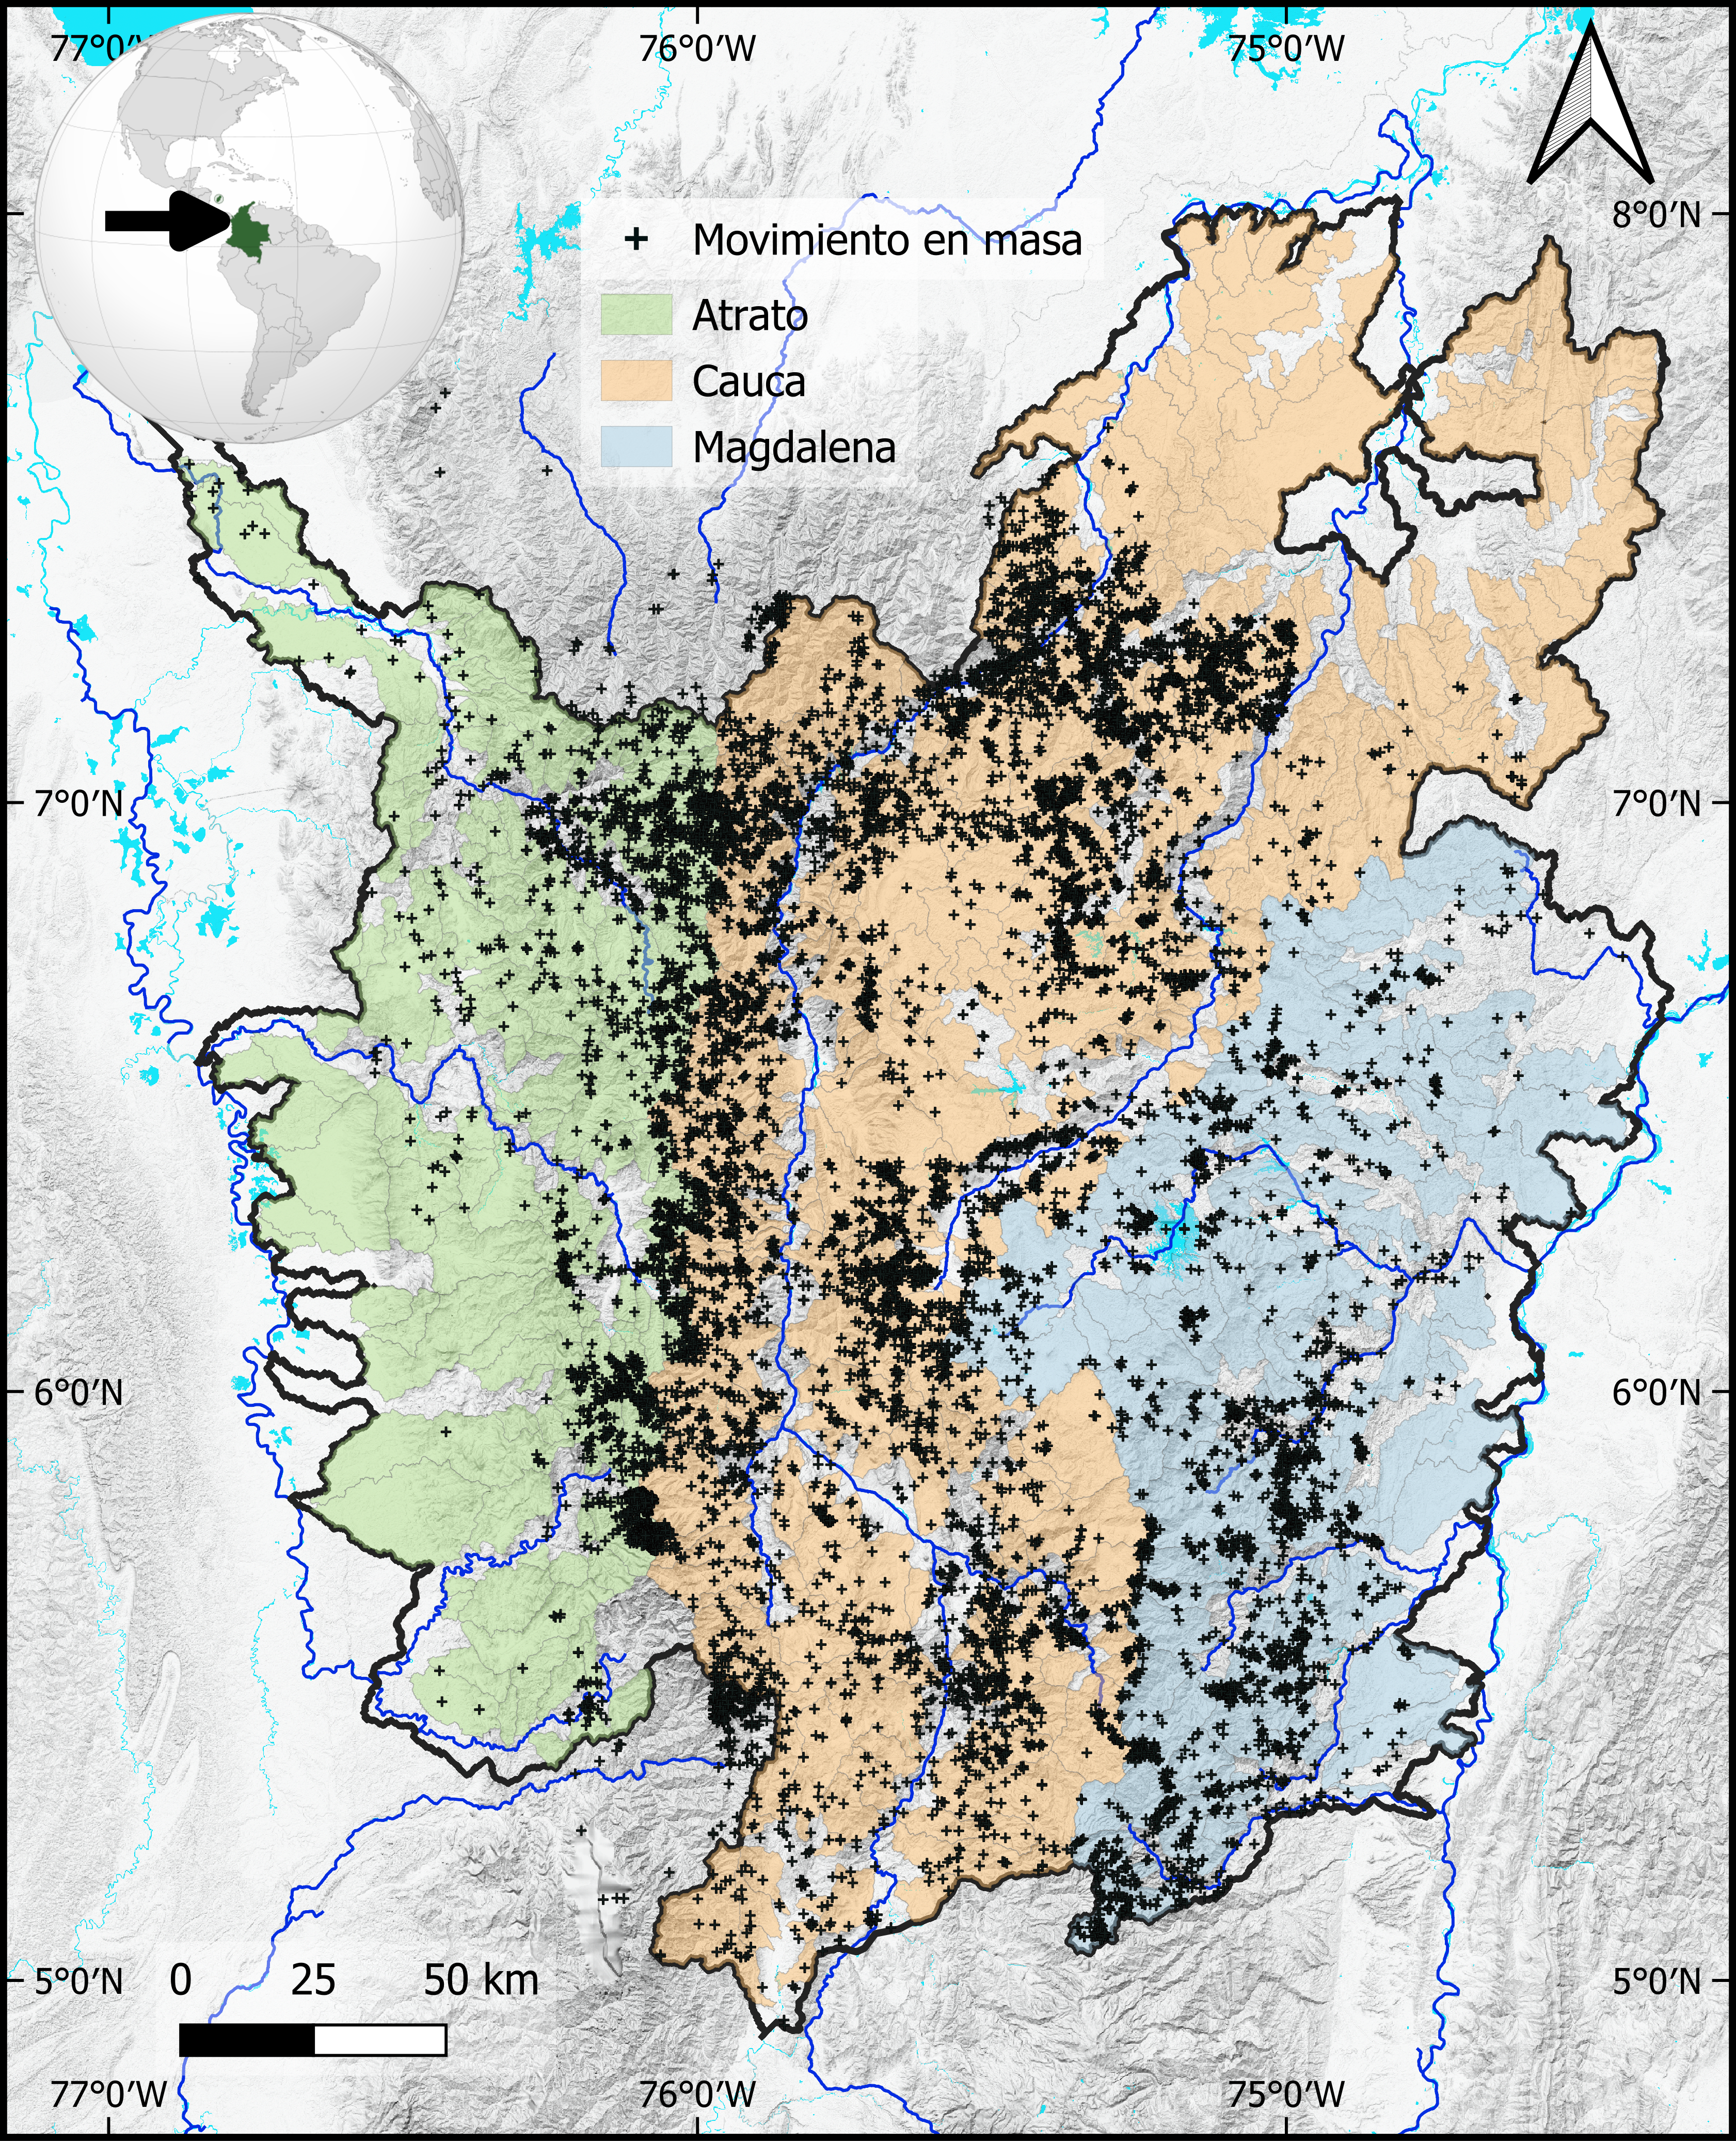
\includegraphics[width=0.7\textwidth]{figures/localizacion.png}
        \caption{Localización del área de estudio en la región andina de Colombia, mostrando la división en las cuencas del Atrato (verde), Cauca (naranja) y Magdalena (azul). Los deslizamientos registrados entre 1970 y 2023 se representan mediante cruces negras.}
        \label{fig:location}
\end{figure}

\par Para el estudio se utilizó un catálogo de 13,777 movimientos en masa que ocurrieron entre 1970 y 2023, los cuales fueron detectados manualmente usando imágenes ópticas en color verdadero de alta resolución ($<$1~m) de Google Earth™. Como variable dependiente se utilizó la frecuencia de movimientos en masa, y como variables predictoras la elevación media ($E$) de la cuenca, el relieve local medio ($H$), la precipitación anual media ($P$) y el área de la cuenca ($A$). Todos los parámetros del terreno se calcularon utilizando el modelo digital de elevación (DEM) del Radar de Apertura Sintética en Banda L del Satélite de Observación Avanzada de la Tierra - Arreglo en Fase (ALOS-PALSAR), con una resolución de píxel de 12.5m \cite{logan2014}. los datos de precipitación se obtuvieron del Grupo CHIRPS ( por sus siglas en ingles Climate Hazard Infrared Precipitation Sensors) \cite{funk2015}, versión 2.0, para datos de precipitación de resolución de 5 km desde 1981 hasta 2023.

\par Para evaluar la dependencia espacial usamos la librería PySAL (\cite{pysal2007}) en Python y los modelos fueron implementados en \textit{spatialreg} (\cite{bivand2022}) en lenguaje R. Para evaluar la bondad de ajuste y comparar diferentes modelos, utilizamos el Criterio de Información de Akaike (AIC), donde el modelo con el AIC más bajo logra el mejor equilibrio entre ajuste y complejidad.

\section{Resultados}
La Tabla \ref{tab:lm_summary} presentada el resumen de los resultados obtenidos para el modelo clásico sin considerar la dependencia espacial, proporcionando una referencia inicial para evaluar la efectividad de los modelos posteriores que incorporan la dependencia espacial. Las variables Área, Hipso y Pendiente presentan coeficientes positivos y significativos, lo que indica una relación positiva con la frecuencia de movimientos en masa. Por otro lado, la variable Lluvia muestra un coeficiente negativo significativo, lo cual sugiere que un aumento en la precipitación promedio anual está correlacionado con una menor ocurrencia de deslizamientos. Adicionalmente, la tabla incluye tres pruebas clave para evaluar la estructura espacial de los residuales: el índice de Moran, y las pruebas del Multiplicador de Lagrange para los errores (Error) y la autoregresión espacial de la variable respuesta (Lag). El valor del índice de Moran para los residuales es 0.39, lo cual indica una autocorrelación espacial positiva en los residuos del modelo, sugiriendo que existe un patrón espacial que el modelo base no ha logrado capturar adecuadamente. Los valores elevados en las pruebas LM para Error (316.04) y Lag (276.76) respaldan esta observación, indicando la presencia de una dependencia espacial significativa que debe ser modelada, con un valor mayor para el término del error, lo que sugiere la implementación de un modelo SEM.

\begin{table}[ht]
\centering
\begin{tabular}{lrrrr}
  \hline
Parámetro & Coeficiente & Std. Error & t-value & p-value \\ 
  \hline
(Intercepto) & 1.84 & 0.05 & 36.72 & 0.00 \\ 
  Área & 0.62 & 0.05 & 12.33 & 0.00 \\ 
  Hipso & 0.14 & 0.06 & 2.47 & 0.01 \\ 
  Pendiente & 0.69 & 0.05 & 12.50 & 0.00 \\ 
  Lluvia & -0.29 & 0.05 & -5.34 & 0.00 \\
  \hline 
  I. Moran (Residuales) & 0.39 &  &  &  \\ 
  LM Test (Error) & 316.04 &  &  &  \\ 
  LM Test (Lag) & 276.76 &  &  &  \\ 
   \hline
\end{tabular}
\caption{Resumen del modelo base sin dependencia espacial. Se muestran los coeficientes estimados, errores estándar, valores t y valores p para los parámetros del modelo. Además, se incluyen los resultados del índice de autocorrelación espacial de Moran para los residuales, así como las pruebas LM del Multiplicador de Lagrange para los errores y la autoregresión espacial.} 
\label{tab:lm_summary}
\end{table}

La Figura \ref{fig:base} presenta los resultados del modelo base. En el panel izquierdo se presentan diagramas de caja de los residuales agrupados por cuenca hidrográfica (Atrato, Cauca y Magdalena). Aunque los valores medianos se encuentran relativamente próximos a cero, se puede observar la presencia de diferencias en la variabilidad de los residuales entre las tres cuencas, lo cual sugiere que las características espaciales de cada cuenca podrían estar influyendo en el comportamiento de los residuales. En el panel derecho se presenta la distribución espacial de los valores estimados por el modelo para cada subcuenca. Estos resultados indican que el modelo base, al no incorporar la dependencia espacial, podría estar omitiendo componentes importantes que explican la variación en la susceptibilidad a movimientos en masa.

\begin{figure}[ht!]
    \centering
        \centering
        \includegraphics[width=1\textwidth]{figures/modelo_base.png}
        \caption{Resultados del modelo base sin dependencia espacial. El panel izquierdo presenta diagramas de caja de los residuales agrupados por cuenca hidrográfica (Atrato, Cauca y Magdalena), indicando diferencias en la variabilidad entre cuencas. El panel derecho muestra la distribución espacial de los valores estimados por el modelo en cada subcuenca, utilizando un esquema de colores donde los tonos rojos indican valores estimados más altos de deslizamientos y los tonos azules y verdes representan valores más bajos.}
        \label{fig:base}
\end{figure}

El primer paso para incluir la dependencia espacial es establecer la relación entre las observaciones mediante la matriz de vecindad. La Figura \ref{fig:matrix} presenta un ejemplo de la matriz de vecindad generada para el área de estudio, utilizando el criterio de distancia con un umbral de 20 km. El patrón de conectividad resultante resalta áreas con mayor densidad de conexiones, especialmente en la parte central de la región de estudio, donde el área de las cuencas es más pequeña y existe mayor proximidad entre unidades. Estas áreas con mayor número de vecinos indican una interacción espacial más fuerte.

\begin{figure}[ht!]
    \centering
      {\includegraphics[width=1\textwidth]{figures/Matriz_vecindad.png}}
\caption{Ejemplo de la matriz de vecindad del área de estudio, basada en el criterio de distancia con valor de 20 km. Los puntos azules representan los centroides de las subcuencas y las líneas rojas indican las conexiones entre subcuencas consideradas vecinas dentro del umbral de 20 km.}
    \label{fig:matrix}
\end{figure}

La Figura \ref{fig:area_moran} muestra los resultados del análisis del índice de Moran para la variable área de la cuenca, con la matriz de vecindad previamente obtenida. La línea negra indica el ajuste lineal que se corresponde con el cálculo del índice de Moran, el cual tiene un valor de 0.1. Este valor positivo, aunque relativamente bajo, indica una ligera autocorrelación espacial, sugiriendo que las áreas de las subcuencas están moderadamente correlacionadas con las áreas de sus subcuencas vecinas.

\begin{figure}[ht!]
    \centering
      {\includegraphics[width=1\textwidth]{figures/area_moran.png}}
\caption{Análisis del índice de Moran para la variable Área de la cuenca con una matriz de vecindad con una distancia de 20 km. El panel derecho muestra el mapa de las subcuencas clasificadas en cuatro cuadrantes del diagrama de dispersión de Moran: Q1 (alto-alto, rojo), Q2 (bajo-alto, azul claro), Q3 (bajo-bajo, azul) y Q4 (alto-bajo, rosado), los colores en gris representan observaciones que no son estadísticamente significativas. El panel derecho presenta el diagrama de dispersión de Moran, donde la línea negra indica el índice de Moran (MI = 0.1), sugiriendo una ligera autocorrelación espacial para el área de las subcuencas.}
    \label{fig:area_moran}
\end{figure}

La Figura \ref{fig:hypso_moran} presenta el análisis del índice de Moran para la variable Curva Hipsométrica. El índice de Moran es 0.39, un valor que indica una autocorrelación espacial moderada. Los puntos en el cuadrante Q1 (alto-alto) y Q3 (bajo-bajo) destacan la existencia de subcuencas que tienden a agruparse con características hipsométricas similares.

\begin{figure}[ht!]
    \centering
      {\includegraphics[width=1\textwidth]{figures/hypso_inte_moran.png}}
\caption{Análisis del índice de Moran para la variable Curva Hipsométrica con una matriz de vecindad con una distancia de 20 km.}
    \label{fig:hypso_moran}
\end{figure}

La Figura \ref{fig:slope_moran} presenta el análisis del índice de Moran para la variable pendiente media de las subcuencas. Este patrón sugiere una clara tendencia espacial, con áreas de alta pendiente agrupadas en ciertas partes de la región de estudio. El índice de Moran obtenido es 0.81, un valor elevado que indica una fuerte autocorrelación espacial.

\begin{figure}[ht!]
    \centering
      {\includegraphics[width=1\textwidth]{figures/slope_mean_moran.png}}
\caption{Análisis del índice de Moran para la variable pendiente media de la subcuenca con una matriz de vecindad con una distancia de 20 km.}
    \label{fig:slope_moran}
\end{figure}

La Figura \ref{fig:rainfall_moran} presenta el análisis del índice de Moran para la variable precipitación media anual de las subcuencas. Este patrón espacial es muy evidente en la región de estudio, lo cual indica una tendencia clara en la distribución de la precipitación. El índice de Moran (0.91) sugiere una autocorrelación espacial muy fuerte. Los puntos del cuadrante Q1 están claramente separados, lo cual muestra una agrupación fuerte de áreas con alta precipitación, y los del cuadrante Q3 muestran una relación similar para áreas con baja precipitación.

\begin{figure}[ht!]
    \centering
      {\includegraphics[width=1\textwidth]{figures/rainfallAnnual_mean_moran.png}}
\caption{Análisis del índice de Moran para la variable precipitación media anual con una matriz de vecindad con una distancia de 20 km.}
    \label{fig:rainfall_moran}
\end{figure}

La Figura \ref{fig:slope_distance} presenta los diagramas de dispersión de Moran para la variable pendiente media, evaluados con diferentes matrices de vecindad basadas en distancias de 5, 10, 20, 50 y 100 km. Cada gráfico muestra cómo varía la autocorrelación espacial de la pendiente en función del criterio de distancia utilizado para definir los vecinos. A medida que aumenta la distancia, se observa una disminución gradual en el valor del índice de Moran (MI), que pasa de 0.95 en la distancia de 5 km a 0.37 en la distancia de 100 km. Esta tendencia indica que, para distancias menores, existe una fuerte autocorrelación espacial, lo cual significa que las subcuencas con pendientes similares tienden a estar muy próximas. Conforme la distancia aumenta, la autocorrelación se debilita, sugiriendo que la influencia de la pendiente media disminuye a medida que se consideran subcuencas más distantes entre sí.

\begin{figure}[ht!]
    \centering
      {\includegraphics[width=1\textwidth]{figures/slope_mean_moran_scatter.png}}
\caption{Diagramas de dispersión de Moran para la variable pendiente media, utilizando matrices de vecindad basadas en diferentes distancias (5, 10, 20, 50 y 100 km).}
    \label{fig:slope_distance}
\end{figure}

La Figura \ref{fig:moran_vecinos} presenta el cambio en el índice de Moran para cada variable predictora. Cada gráfico evalúa el índice de Moran utilizando matrices de vecindad basadas en distancias que van desde 5 km hasta 200 km, aumentando cada 5 km. La figura señala cómo cambia la autocorrelación espacial de cada variable a medida que se expande el radio de influencia entre subcuencas. Además, cada punto está etiquetado con el porcentaje de observaciones (subcuencas) que muestran resultados estadísticamente significativos, lo cual proporciona una visión adicional sobre la consistencia de la autocorrelación espacial a diferentes escalas.

Para el área de la cuenca (superior izquierda) se observa una disminución rápida del índice de Moran conforme aumenta la distancia. El porcentaje de subcuencas con resultados estadísticamente significativos es relativamente bajo, con un máximo del 17\% en distancias cortas y disminuyendo rápidamente, lo cual indica que la autocorrelación espacial del área es moderada y de alcance local. Para la variable curva hipsométrica (superior derecha)) el índice de Moran comienza en valores más elevados (alrededor de 0.6) y disminuye gradualmente hasta 0.2. La autocorrelación espacial para esta variable se mantiene significativa en una mayor proporción de subcuencas (hasta 41\% en distancias cortas), lo cual sugiere que la distribución de la hipsometría tiene un patrón más robusto y generalizado en el área de estudio. Para la precipitación media anual (inferior derecha)) se observa inicialmente un índice de Moran cercano a 1, lo cual indica una fuerte autocorrelación espacial que se diluye lentamente a medida que aumenta la distancia, pero aún mantiene valores relativamente altos (> 0.5) incluso a mayores distancias. El porcentaje de subcuencas con resultados significativos es también muy alto (> 60\%), lo cual refleja la homogeneidad espacial de la precipitación en el área de estudio. Finalmente, para la pendiente media (inferior izquierda) el índice de Moran para la pendiente también comienza en valores altos, alrededor de 0.95, y disminuye conforme aumenta la distancia, aunque sigue siendo significativo hasta distancias intermedias. El porcentaje de subcuencas con resultados significativos es alto en distancias cortas (hasta 53\%) y luego disminuye gradualmente, indicando que la pendiente tiene una fuerte correlación espacial local que se debilita lentamente.

\begin{figure}[ht!]
    \centering
    \begin{minipage}{0.48\textwidth}
        \centering
        \includegraphics[width=\textwidth]{figures/area_moran_vs_distance.png}
    \end{minipage}%
    \hfill
    \begin{minipage}{0.48\textwidth}
        \centering
        \includegraphics[width=\textwidth]{figures/hypso_inte_moran_vs_distance.png}
    \end{minipage}
    
    \vspace{0.5cm} % Adjust vertical spacing between rows as needed
    
    \begin{minipage}{0.48\textwidth}
        \centering
        \includegraphics[width=\textwidth]{figures/slope_mean_moran_vs_distance.png}
    \end{minipage}%
    \hfill
    \begin{minipage}{0.48\textwidth}
        \centering
        \includegraphics[width=\textwidth]{figures/rainfallAnnual_mean_moran_vs_distance.png}
    \end{minipage}
    \label{moran_vecinos}
     \caption{Cambios en el índice de Moran para las variables Área de la Cuenca (superior derecha)), Curva Hipsométrica (superior izquierda), Precipitación Media Anual (inferior derecha) y Pendiente Media (inferior izquierda), utilizando matrices de vecindad basadas en distancias de 5 km a 200 km, con incrementos de 5 km. Cada punto muestra el porcentaje de subcuencas con resultados estadísticamente significativos.}
\end{figure}

La Figura \ref{fig:moran_distancia} presenta  el índice de Moran utilizando como matriz de vecindad el criterio de los vecinos más cercanos, con valores de K variando entre 1 y 200. El índice de Moran para el área de la cuenca comienza en valores bajos (aproximadamente 0.2) cuando se consideran pocos vecinos (K = 1), y disminuye rápidamente hasta alcanzar casi cero para valores de K superiores. El porcentaje de subcuencas con resultados significativos también es bajo, alcanzando un máximo de 17\%. La autocorrelación espacial para la variable hipsométrica muestra valores iniciales del índice de Moran más altos (cercanos a 0.6) cuando se consideran pocos vecinos, lo cual decrece gradualmente hasta alcanzar valores cercanos a cero para K mayores a 100. El porcentaje de significancia es mayor en comparación con el área, alcanzando hasta un 42\%. El índice de Moran para la precipitación es inicialmente muy alto, cercano a 1, disminuyendo de forma sostenida conforme aumenta K. Para la pendiente media, el índice de Moran también comienza con valores elevados (alrededor de 0.95), y se reduce de manera constante a medida que se incrementa K. El porcentaje de subcuencas con significancia estadística es alto (más del 80\%) para valores pequeños de K y disminuye progresivamente.

\begin{figure}[ht!]
    \centering
    \begin{minipage}{0.48\textwidth}
        \centering
        \includegraphics[width=\textwidth]{figures/area_moran_vs_k_neighbors.png}
    \end{minipage}%
    \hfill
    \begin{minipage}{0.48\textwidth}
        \centering
        \includegraphics[width=\textwidth]{figures/hypso_inte_moran_vs_k_neighbors.png}
    \end{minipage}
    
    \vspace{0.5cm} % Adjust vertical spacing between rows as needed
    
    \begin{minipage}{0.48\textwidth}
        \centering
        \includegraphics[width=\textwidth]{figures/slope_mean_moran_vs_k_neighbors.png}
    \end{minipage}%
    \hfill
    \begin{minipage}{0.48\textwidth}
        \centering
        \includegraphics[width=\textwidth]{figures/rainfallAnnual_mean_moran_vs_k_neighbors.png}
        \label{fig:moran_distancia}
    \end{minipage}
            \caption{Cambios en el índice de Moran para las variables Área de la Cuenca, Curva Hipsométrica, Precipitación Media Anual y Pendiente Media, utilizando matrices de vecinos más cercanos (KNN) con valores de K entre 1 y 10 (incrementos de 1) y de 10 hasta 200 (incrementos de 5). Cada punto muestra el valor del índice de Moran y el porcentaje de subcuencas con resultados estadísticamente significativos.}
\end{figure}

La Tabla \ref{tab:spatial_models} presenta los resultados de los modelos espaciales que incluyen la dependencia espacial en la modelación de la ocurrencia de movimientos en masa: SAR (\textit{Spatial Autoregressive Model}), SEM (\textit{Spatial Error Model}), SAC (\textit{Spatial Autoregressive Combined Model}), SLX (\textit{Spatial Lagged X Model}), SDEM (\textit{Spatial Durbin Error Model}), SDM (\textit{Spatial Durbin Model}), y GNS (\textit{General Nesting Spatial Model}). La variable curva hipsométrica tiene un coeficiente positivo y significativo en todos los modelos, lo que sugiere que tiene un efecto robusto en la ocurrencia de deslizamientos. Por otro lado, la variable Lluvia presenta un efecto negativo en la mayoría de los modelos, aunque en algunos casos sin alcanzar la significancia. Además, se presentan los coeficientes asociados a las dependencias espaciales, como $\rho$ (autocorrelación espacial en la variable dependiente) y $\lambda$ (autocorrelación en los errores). Los valores de $\rho$ y $\lambda$ son elevados en los modelos SAR y SEM, respectivamente, indicando que la dependencia espacial está capturando efectos importantes no modelados por los predictores. También se incluye el parámetro $Wx$ para las variables explicativas en los modelos que consideran interacciones espaciales con los predictores (SLX, SDEM, SDM, y GNS). El modelo SAC tiene el menor valor de AIC (1455), lo cual sugiere que este modelo ofrece el mejor equilibrio entre ajuste y complejidad, seguido de cerca por el SDEM (1460) con un $R^2$ ligeramente mayor.

\begin{table}[ht]
\centering
\begin{tabular}{llllllll}
   \hline
 Parámetro & SAR & SEM & SAC & SLX & SDEM & SDM & GNS \\ 
  \hline
Intercepto & \textbf{0.651} (0.08) & \textbf{1.819} (0.14) & \textbf{1.129} (0.23) & \textbf{1.859} (0.05) & \textbf{1.823} (0.14) & \textbf{0.549} (0.08) & \textbf{1.558} (0.52) \\ 
  Área & \textbf{0.105} (0.05) & \textbf{0.106} (0.05) & \textbf{0.106} (0.05) & 0.101 (0.06) & \textbf{0.105} (0.05) & \textbf{0.103} (0.05) & \textbf{0.106} (0.05) \\ 
  Hipso & \textbf{0.556} (0.04) & \textbf{0.588} (0.04) & \textbf{0.594} (0.04) & \textbf{0.592} (0.05) & \textbf{0.603} (0.04) & \textbf{0.587} (0.04) & \textbf{0.601} (0.04) \\ 
  Pendiente & \textbf{0.295} (0.05) & \textbf{0.534} (0.08) & \textbf{0.452} (0.09) & \textbf{0.477} (0.13) & \textbf{0.415} (0.10) & \textbf{0.411} (0.10) & \textbf{0.407} (0.10) \\ 
  Lluvia & \textbf{-0.106} (0.05) & \textbf{-0.380} (0.11) & \textbf{-0.211} (0.09) & \textbf{-0.636} (0.30) & -0.452 (0.27) & -0.445 (0.24) & -0.452 (0.27) \\ 
     \hline
  Wx-Área &  &  &  & 0.185 (0.12) & 0.066 (0.16) & -0.012 (0.10) & 0.060 (0.15) \\ 
  Wx-Hipso &  &  &  & \textbf{0.290} (0.14) & 0.209 (0.16) & \textbf{-0.280} (0.12) & 0.124 (0.23) \\ 
Wx-Pendiente &  &  &  & 0.238 (0.15) & \textbf{0.387} (0.17) & -0.170 (0.13) & 0.273 (0.25) \\ 
  Wx-Lluvia &  &  &  & 0.433 (0.32) & 0.173 (0.33) & 0.380 (0.26) & 0.226 (0.33) \\ 
   \hline
$\rho$ & 0.657 &  & 0.388 &  &  & 0.702 & 0.148 \\ 
  $\lambda$ &  & 0.716 & 0.464 &  & 0.708 &  & 0.636 \\ 
  Nagelkerke $R^2$ & 0.624 & 0.627 & 0.631 &  & 0.632 & 0.631 & 0.633 \\ 
  AIC & 1464.141 & 1460.692 & 1455.857 & 1642.684 & 1460.333 & 1461.73 & 1461.973 \\ 
     \hline
  \end{tabular}
\caption{Resultados de diferentes modelos espaciales aplicados para la susceptibilidad por movimientos en masa. Se presentan los coeficientes estimados (con errores estándar entre paréntesis y significado estadístico en negrilla) para las variables Área, Hipso, Pendiente y Lluvia, así como los coeficientes espaciales $\rho$ y $\lambda$. También se pressenta el ajuste del modelo a través del coeficiente de Nagelkerke $R^2$ y el AIC.} 
\label{tab:spatial_models}
\end{table}

La Tabla \ref{tab:sdem_summary} presenta los resultados del modelo SDEM considerando matrices de vecindad basadas en distancias de 20, 40, 60, 80, y 100 km. A medida que aumenta la distancia de vecindad, se observa una reducción en la magnitud y significancia de varios parámetros. Por ejemplo, el intercepto disminuye de un valor significativo en 20 km ($1.82$) a valores no significativos a partir de los 60 km, sugiriendo que la capacidad del modelo para capturar patrones consistentes disminuye con el incremento de la distancia. La variable área de la cuenca mantiene un coeficiente significativo en todas las distancias, lo cual destaca su relevancia en la explicación de la ocurrencia de deslizamientos. La variable hipso muestra un coeficiente positivo que pierde significancia conforme aumenta la distancia, mientras que la pendiente presenta un coeficiente positivo y significativo en todas las distancias, lo cual indica que la pendiente sigue siendo un factor importante de acuerdo con el alcance espacial considerado. La variable lluvia, por otro lado, muestra un comportamiento mixto, siendo significativa solo en la distancia de 60 km y pasando a no ser significativa a mayores distancias. En cuanto a los efectos espaciales ($Wx$), los coeficientes correspondientes a las variables predictoras muestran una alta variabilidad. El coeficiente de la pendiente autoregresion espacial ($Wx-Pendiente$) es significativo para la distancia de 20 km, lo que sugiere que la influencia de la pendiente en las subcuencas vecinas se percibe a esta escala. El coeficiente de Nagelkerke $R^2$ disminuye conforme aumenta la distancia, lo cual indica una reducción en la capacidad explicativa del modelo con el incremento de la vecindad. El AIC también aumenta progresivamente a medida que aumenta la distancia, lo que refleja la reducción del ajuste del modelo. Se observa que para distancias mayores a 20 km, los valores de MI aumentan y sus $p$-valores se tornan significativos ($p$ < 0.05), sugiriendo la presencia de autocorrelación residual que no está siendo capturada por el modelo.

\begin{table}[ht]
\centering
\begin{tabular}{llllll}
  \hline
Parámetro & 20km & 40km & 60km & 80km & 100km \\ 
  \hline
Intercepto & \textbf{1.82} (0.14) & \textbf{1.74} (0.32) & \textbf{1.66} (0.54) & 1.42 (0.87) & 1.29 (1.03) \\ 
  Área & \textbf{0.60} (0.04) & \textbf{0.57} (0.04) & \textbf{0.57} (0.04) & \textbf{0.57} (0.05) & \textbf{0.57} (0.05) \\ 
  Hipso & \textbf{0.11} (0.05) & 0.09 (0.05) & 0.09 (0.05) & 0.09 (0.05) & 0.08 (0.05) \\ 
  Pendiente & \textbf{0.42} (0.10) & \textbf{0.43} (0.10) & \textbf{0.53} (0.09) & \textbf{0.56} (0.09) & \textbf{0.51} (0.09) \\ 
  Lluvia & -0.45 (0.27) & -0.24 (0.20) & \textbf{-0.40} (0.16) & -0.21 (0.17) & 0.00 (0.17) \\ 
  Wx-Área & 0.21 (0.16) & -0.44 (0.38) & 0.43 (0.53) & 0.96 (0.71) & 1.29 (0.86) \\ 
  Wx-Hipso & 0.07 (0.16) & -0.04 (0.32) & -0.02 (0.42) & 0.04 (0.50) & 0.44 (0.54) \\ 
  Wx-Pendiente & \textbf{0.39} (0.17) & 0.50 (0.27) & 0.41 (0.34) & 0.34 (0.42) & 0.41 (0.45) \\ 
  Wx-Lluvia & 0.17 (0.33) & -0.06 (0.36) & 0.33 (0.36) & -0.05 (0.47) & -0.73 (0.63) \\ 
  $\lambda$ & 0.708 & 0.871 & 0.919 & 0.949 & 0.957 \\ 
      \hline
  Nagelkerke $R^2$ & 0.632 & 0.616 & 0.59 & 0.574 & 0.568 \\ 
  AIC & 1460.333 & 1482.916 & 1518.336 & 1537.402 & 1545.834 \\ 
  MI & 0.006 & 0.026 & 0.031 & 0.04 & 0.041 \\ 
  $p$-value Moran & 0.361 & 0.015 & 0.001 & 0.001 & 0.001 \\ 
   \hline
\end{tabular}
\caption{Resultados del modelo SDEM para diferentes distancias de vecindad. Se presentan los coeficientes estimados (con errores estándar entre paréntesis) para las variables predictoras, junto con los coeficientes espaciales ($Wx$) y el coeficiente de autocorrelación en los errores ($\lambda$). También se muestran el coeficiente de Nagelkerke $R^2$, el AIC, el índice de Moran (MI) y su $p$-valor} 
\label{tab:sdem_summary}
\end{table}

La Figura \ref{fig:residuals_fitted} presenta los resultados del modelo SDEM con los residuales del modelo agrupados por cuencas hidrográficas y la distribución espacial de los valores estimados para cada subcuenca en el área de estudio. En los diagramas de caja, se observa que la mediana de los residuales en las tres cuencas se encuentra cerca de cero, lo cual indica que el modelo no presenta un sesgo significativo. 

\begin{figure}[ht!]
    \centering
      {\includegraphics[width=1\textwidth]{figures/Residuals_and_Fitted_Values.png}}
\caption{Resultados del modelo SDEM. El panel izquierdo muestra diagramas de caja de los residuales agrupados por cuenca hidrográfica (Atrato, Cauca y Magdalena), indicando la variabilidad y presencia de valores atípicos. El panel derecho presenta la distribución espacial de los valores estimados de deslizamientos por subcuenca, con un esquema de colores que varía de tonos bajos (morado) a altos (rojo).}
    \label{fig:residuals_fitted}
\end{figure}

\section{Discusión}

Durante muchas décadas, se ha reconocido el componente espacial de los datos, especialmente en disciplinas relacionadas con la geografía, econometría y epidemiología (\cite{anselin2022spatial, rey2023geographic}). Sin embargo, en la práctica, la incorporación efectiva de este componente en los modelos estadísticos ha sido limitada. Solo recientemente, con los avances acelerados en la captura de datos espaciales, mediante el sensoramiento remoto y el Internet de las cosas (IoT), así como con el aumento de la capacidad de almacenamiento y procesamiento de los ordenadores, se han desarrollado técnicas que permiten abordar de forma más adecuada la espacialidad de los datos. Estos avances han facilitado la implementación de modelos geoespaciales más robustos, como los modelos de autoregresión espacial (\cite{wall2004close}), los modelos multiniveles (\cite{lee1996hierarchical}) o los procesos Gaussianos (\cite{vasudevan2009gaussian}), que permiten incorporar la estructura espacial inherente a los fenómenos naturales.

La omisión de la estructura espacial en modelos estadísticos clásicos puede generar resultados sesgados o no representativos, ya que dichos modelos generalmente asumen independencia entre las observaciones (\cite{anselin1988spatial, lesage2011pitfalls}). Esta estructura espacial en los datos viola supuestos básicos de los modelos de regresión clásica, como la independencia de los residuos, la homocedasticidad (varianza constante de los residuos), y la ausencia de multicolinealidad entre los predictores (\cite{cressie1988spatial, ripley1988statistical, anselin1988spatial}). El impacto de la dependencia espacial en las pruebas estadísticas y en las medidas de ajuste puede ser engañoso debido a la estimación sesgada de la varianza del error, los niveles de significancia de las pruebas $T$ y los valores de $R^2$ (\cite{anselin1990spatial}).

Tener una estructura espacial significa que los datos exhiben una correlación debido a su proximidad en el espacio, lo que resulta en patrones que deben ser adecuadamente modelados. La heterogeneidad espacial, que se refiere a la variación en las propiedades a lo largo del espacio, y la dependencia espacial, que implica que los valores en ubicaciones cercanas tienden a estar correlacionados, son las estructuras espaciales mas comunes descritas en la literatura (\cite{anselin1988spatial, rey2023geographic}). La dependencia espacial es observada en procesos naturales; por ejemplo, en el caso de los movimientos en masa, las áreas con alta susceptibilidad tienden a influir en áreas vecinas debido a la continuidad de factores como la pendiente, la litología y la cobertura del suelo (\cite{samia2019dynamic}). Esto implica que un evento en una ubicación específica puede aumentar la probabilidad de ocurrencia en ubicaciones cercanas, generando patrones espaciales de correlación que los modelos deben incorporar.

La naturaleza espacial de los datos exige la implementación de modelos que puedan manejar explícitamente esta característica. En el presente estudio, utilizamos modelos de regresi@on espacial para abordar la dependencia espacial de manera adecuada. Los modelos SAR permiten capturar dicha dependencia a través de una matriz de vecindad, la cual puede definirse según criterios de contigüidad o distancia. Los resultados señalan cómo la elección del criterio de vecindad tiene un impacto directo en los resultados del modelo, ya que determina cómo se representan las interacciones espaciales y cómo se propaga la influencia entre las unidades de análisis. Por ejemplo, una matriz basada en la contigüidad puede ser importante cuando los bordes entre las unidades discretas utilizadas controle o determine la interacción entre vecinos. Mientras que una matriz basada en la distancia puede tener en cuenta efectos que se extienden más allá de los límites inmediatos, lo cual puede ser crucial dependiendo del fenómeno estudiado. Para el caso de este estudio, hemos seleccionado trabajar con matrices basadas en distancia, ya que los parámetros morfométricos, como pendiente e hipsometría, así como la precipitación, se manifiestan en el terreno sin seguir un limite o borde establecido. El caso de la precipitación por ejemplo, aunque puede tener influencias del relieve, no presenta limites basados en contigüidad. Por lo tanto una aproximación basada en distancias puede representar de mejor forma el proceso espacial subyacente. Sin embargo, esto debe ser evaluado en cada caso de aplicación.

La inclusión explícita de la dependencia espacial no solo puede mitigar los problemas derivados de la asunción de independencia en los modelos estadísticos convencionales, sino que también aporta información adicional que mejora el desempeño y capacidad predictiva del modelo. En este estudio, la consideración de la dependencia espacial ha mejorado tanto la interpretabilidad como la precisión del modelo, dado que se incorpora la estructura espacial subyacente al fenómeno estudiado. Esto ha permitido una representación que se puede ajustar mejor a los patrones observados y una mejora significativa en la calidad de las predicciones, comparado con los modelos clásicos que no consideran este aspecto fundamental.

Para este estudio se emplearon datos de subcuencas localizadas en los Andes colombianos, junto con variables predictoras morfométricas que operan tanto a escala local como regional. Por ejemplo, se consideraron variables locales como la pendiente, y variables regionales como la precipitación media anual. La combinación de variables con efectos locales o efectos regionales es observada, y en este caso estimadas, para casos como la evaluación de la susceptibilidad por movimientos en masa, lo que contribuye a una comprensión más profunda de la influencia espacial y la estructura del fenómeno.

Los resultados del estudio evidenciaron la presencia de una estructura espacial en función de la distancia para las variables consideradas. En el caso del área de la cuenca, no se identificó una estructura espacial significativa, mientras que la hipsometría de la cuenca mostró una estructura espacial moderada. Por otro lado, las variables de pendiente y precipitación evidenciaron un fuerte componente espacial, con una marcada tendencia a la formación de clústeres de valores altos y bajos.

Para evaluar la dependencia espacial, se analizó el índice de Moran en función de la distancia para todas las variables, considerando la significancia estadística de las observaciones. Se encontró que, al emplear distancias cortas, la correlación espacial aumentaba, pero también lo hacía la varianza, lo cual disminuía la significancia estadística en muchas observaciones. Esto se debe a que un aumento en la varianza introduce una mayor incertidumbre en los estimadores del modelo, lo cual dificulta la detección de patrones significativos y disminuye la capacidad para rechazar hipótesis nulas. A distancias mayores, la correlación espacial disminuía, al igual que la varianza.

Los resultados arrojaron que para la pendiente y la precipitación media anual a medida que aumenta la distancia se reduce la influencia entre las subcuencas, pero a diferentes tasas. Para la pendiente se observa una tasa de reducción menor comparada con la precipitación; mientras que para la precipitación media anual es mayor a dsitancias cortas pero se va reduciendo a mediad que aumenta la distancia. En ambos casos se alcanzan valores alrededor de 0,2 para distancias mayores a 100 km. 

También se implementó el criterio de los vecinos más cercanos para obtener las matrices de vecindad, los resultados indicaron que la matriz basada en distancia capturó de manera más adecuada la dependencia espacial de los datos. Las curvas de la variación del indice de Moran con el número de vecinos mostraron tendencias similares al criterio de distancia, pero con un área bajo la curva menor, indicando una menor capacidad explicativa en comparación con el criterio basado en la distancia.

En cuanto al modelo de regresión clásico, los resultados, junto con el índice de Moran y la prueba de Lagrange, evidenciaron la presencia de estructura espacial en los residuales del modelo. Por tanto, se implementaron modelos de autoregresión espacial. Las matrices espaciales en los modelos SAR permiten la incorporación de la dependencia en las variables exógenas (predictores) o variable endógena (el término de error o la variable respuesta). \cite{lesage2014spatial} propone considerar solo dos modelos espaciales: el SDM y el SDEM. El SDM asume que los efectos de vecindad son globales por que la autoregresión es simultanea al estar en la variable respuesta, mientras que el SDEM se encuentra en el termino del error por lo que se asume que son locales. Los autores recomiendan usar un modelo SEM cuando no haya una comprensión clara del origen del efecto de dependencia (\cite{elhorst2014spatial}). Otra recomendación está en que si no existen razones teóricas que justifiquen un modelo específico, podría ser preferible confiar en la especificación SLX más simple, en lugar de adoptar el modelo más complejo SDM (\cite{halleck2017regional, halleck2015slx}).

En este caso implementamos todos los modelos para comparar sus resultados. Para la construcción de los modelos se utilizó una distancia de 25 km como criterio de vecindad, dado que las variables con mayor dependencia espacial, como la pendiente y la precipitación, presentaban altos niveles de dependencia en este rango, y más del 60\% de los datos mostraban significancia estadística. Esta elección optimizó el equilibrio entre la correlación espacial y la varianza, obteniendo resultados robustos y significativos. Aunque los resultados fueron satisfactorios, cabe mencionar que existen otros criterios para optimizar la matriz de vecindad que no se exploraron en este trabajo. Por ejemplo, el punto de inflexión de la curva de dependencia podría ser utilizado para establecer una distancia óptima en la matriz de vecindad. Este enfoque podría proporcionar una alternativa para representar la estructura espacial de los datos y mejorar la capacidad predictiva del modelo.

La prueba de Lagrange en los residuales del modelo clásico sugirió la incorporación de la dependencia en el término de error, lo cual fue posteriormente confirmado. En términos del coeficiente de determinación ajustado ($R^2$ ajustado) y el criterio de información de Akaike (AIC), los modelos con mejor desempeño fueron el SAC, SEM y el SDEM, con resultados similares, todos ellos comparten en común que el componente de autoregresión es incorporado en el error. Aunque el SDEM presentó un $R^2$ ajustado ligeramente superior.

La incorporación de la estructura espacial mejoró significativamente los resultados en comparación con el modelo clásico, eliminando la estructura espacial de los residuales, lo cual confirma la relevancia de considerar la dependencia espacial en el modelado de fenómenos naturales como los movimientos en masa. Además, el SDEM, que presentó el mejor desempeño, fue utilizado para construir distintas versiones del modelo, modificando la matriz de vecindad en función de la distancia. Se observó que, a medida que aumentaba la distancia para definir la vecindad, los valores de $R^2$ ajustado disminuían, mientras que el índice de Moran en los residuales y el coeficiente de autoregresión del error ($\lambda$) aumentaban de manera significativa.

\section{Conclusiones}

Los hallazgos de este estudio subrayan la importancia de integrar la dependencia espacial en la modelación de la susceptibilidad a movimientos en masa. Los modelos de regresión tradicionales, que generalmente asumen la independencia de las observaciones, no logran capturar adecuadamente la estructura espacial inherente a los procesos geomorfológicos como los movimientos en masa, lo que resulta en estimaciones sesgadas, precisión reducida y conclusiones potencialmente erróneas. Al incorporar la dependencia espacial, los modelos pueden representar de manera más precisa las dinámicas de los movimientos en masa, mejorando así la capacidad predictiva y la fiabilidad de los resultados.

Los modelos autoregresivos espaciales, en particular el Modelo de Error de Durbin Espacial (SDEM), demostraron en nuestra zona de estudio ser efectivos para abordar las interacciones espaciales que los modelos clásicos no logran capturar. El SDEM, que incorpora la dependencia espacial tanto en las variables predictoras como en los residuales, mostró un desempeño superior en varias métricas de evaluación, incluyendo el $R^2$ ajustado y el AIC. Al tener en cuenta los efectos de vecindad locales, el SDEM ofreció una comprensión más integral de cómo factores geoambientales como la pendiente, la precipitación y la hipsometría contribuyen a la susceptibilidad por movimientos en masa.

El estudio también destaca la importancia de seleccionar una matriz de vecindad adecuada. En este caso, una matriz de vecindad basada en la distancia capturó de manera efectiva las dinámicas espaciales de variables clave, como la pendiente y la precipitación anual. Nuestros datos sugieren que el uso de matrices basadas en la distancia proporciona una representación más flexible y precisa de las interacciones espaciales, que no necesariamente se ajustan a límites administrativos o naturales.

Variables como la pendiente y la precipitación mostraron una notable agrupación espacial, lo que hace necesario incluir estos componentes espaciales en los modelos predictivos para mejorar la precisión. El uso del Índice de Moran y las pruebas del Multiplicador de Lagrange validó aún más la necesidad de la modelación espacial, ya que estas pruebas identificaron una autocorrelación espacial sustancial en los residuales de los modelos de regresión tradicionales.

\begin{acknowledgement}
El presente trabajo se realizo con el apoyo de la Fundación Alexander von Humboldt (\url{https://www.humboldt-foundation.de/}) a través del programa \textit{Georg Forster Research Fellowship} para investigadores.

\end{acknowledgement}

\section{Open Research}
Data and code used for this study are fully available in Github (\url{}).

\printbibliography

\end{document}
